\documentclass{standalone}

\usepackage{tikz}
\usepackage{pgfplots}
\usetikzlibrary{calc, tikzmark, shapes, shapes.arrows, arrows, 3d, positioning}
\pgfplotsset{compat=1.17}
\begin{document}
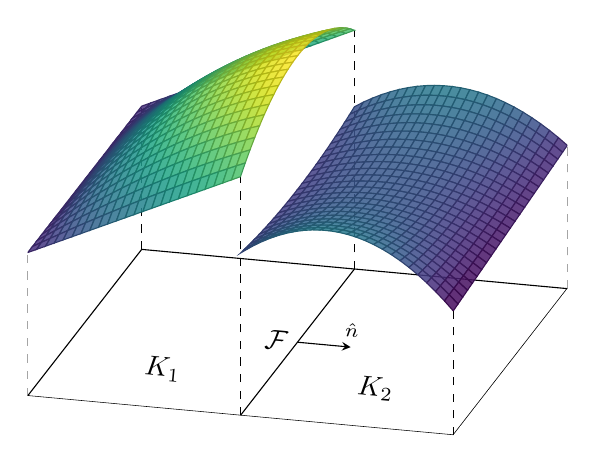
\begin{tikzpicture}
	\begin{axis}[anchor=origin, axis lines=none, xmax=2, ymax=1, zmin=-1, zmax=1.75, colormap/viridis, view={15}{30}]
		\begin{scope}[canvas is xy plane at z=-1]
			\draw (0,0) -- (2,0) -- (2,1) -- (0,1) -- (0,0); 
			\draw (1,0) -- (1,1); 
		\end{scope}
		\begin{scope}[canvas is xy plane at z=-1]
			\node[sloped like x axis] at (.5,.25) {$K_1$}; 
			\node[sloped like x axis] at (1.50,.25) {$K_2$}; 
			\node[sloped like x axis] at (.90,.50) {$\mathcal{F}$}; 
			\draw[->, >=stealth] (1,.5) -- (1.25,.5) node[above,sloped like x axis] {\scriptsize$\hat{n}$}; 
		\end{scope}

		\draw[dashed] (0,0,-1) -- (0,0,.5); 
		\draw[dashed] (0,1,-1) -- (0,1,.5); 
		\draw[dashed] (1,1,-1) -- (1,1,1.50); 
		\draw[dashed] (1,0,-1) -- (1,0,1.50); 
		\addplot3[domain=0:1, y domain=0:1, fill opacity=.85, surf]({x},{y},{1+x*x*y*(-4+4*y) + x*(1+6*y-6*y*y)-.5}); 
		\addplot3[domain=1:2, y domain=0:1, fill opacity=.85, surf]({x},{y},{
			-2.9 + 6.2*y - 5.6*y^2 + x^2*(-2. + 3.6*y - 3.2*y^2) + x*(5.6 - 10.2*y + 9.2*y^2)
		}); 
		\draw[dashed] (2,0,-1) -- (2,0,.30); 
		\draw[dashed] (2,1,-1) -- (2,1,.50); 
	\end{axis}
\end{tikzpicture}
\end{document}